\begin{figure*}[t]
    \centering
    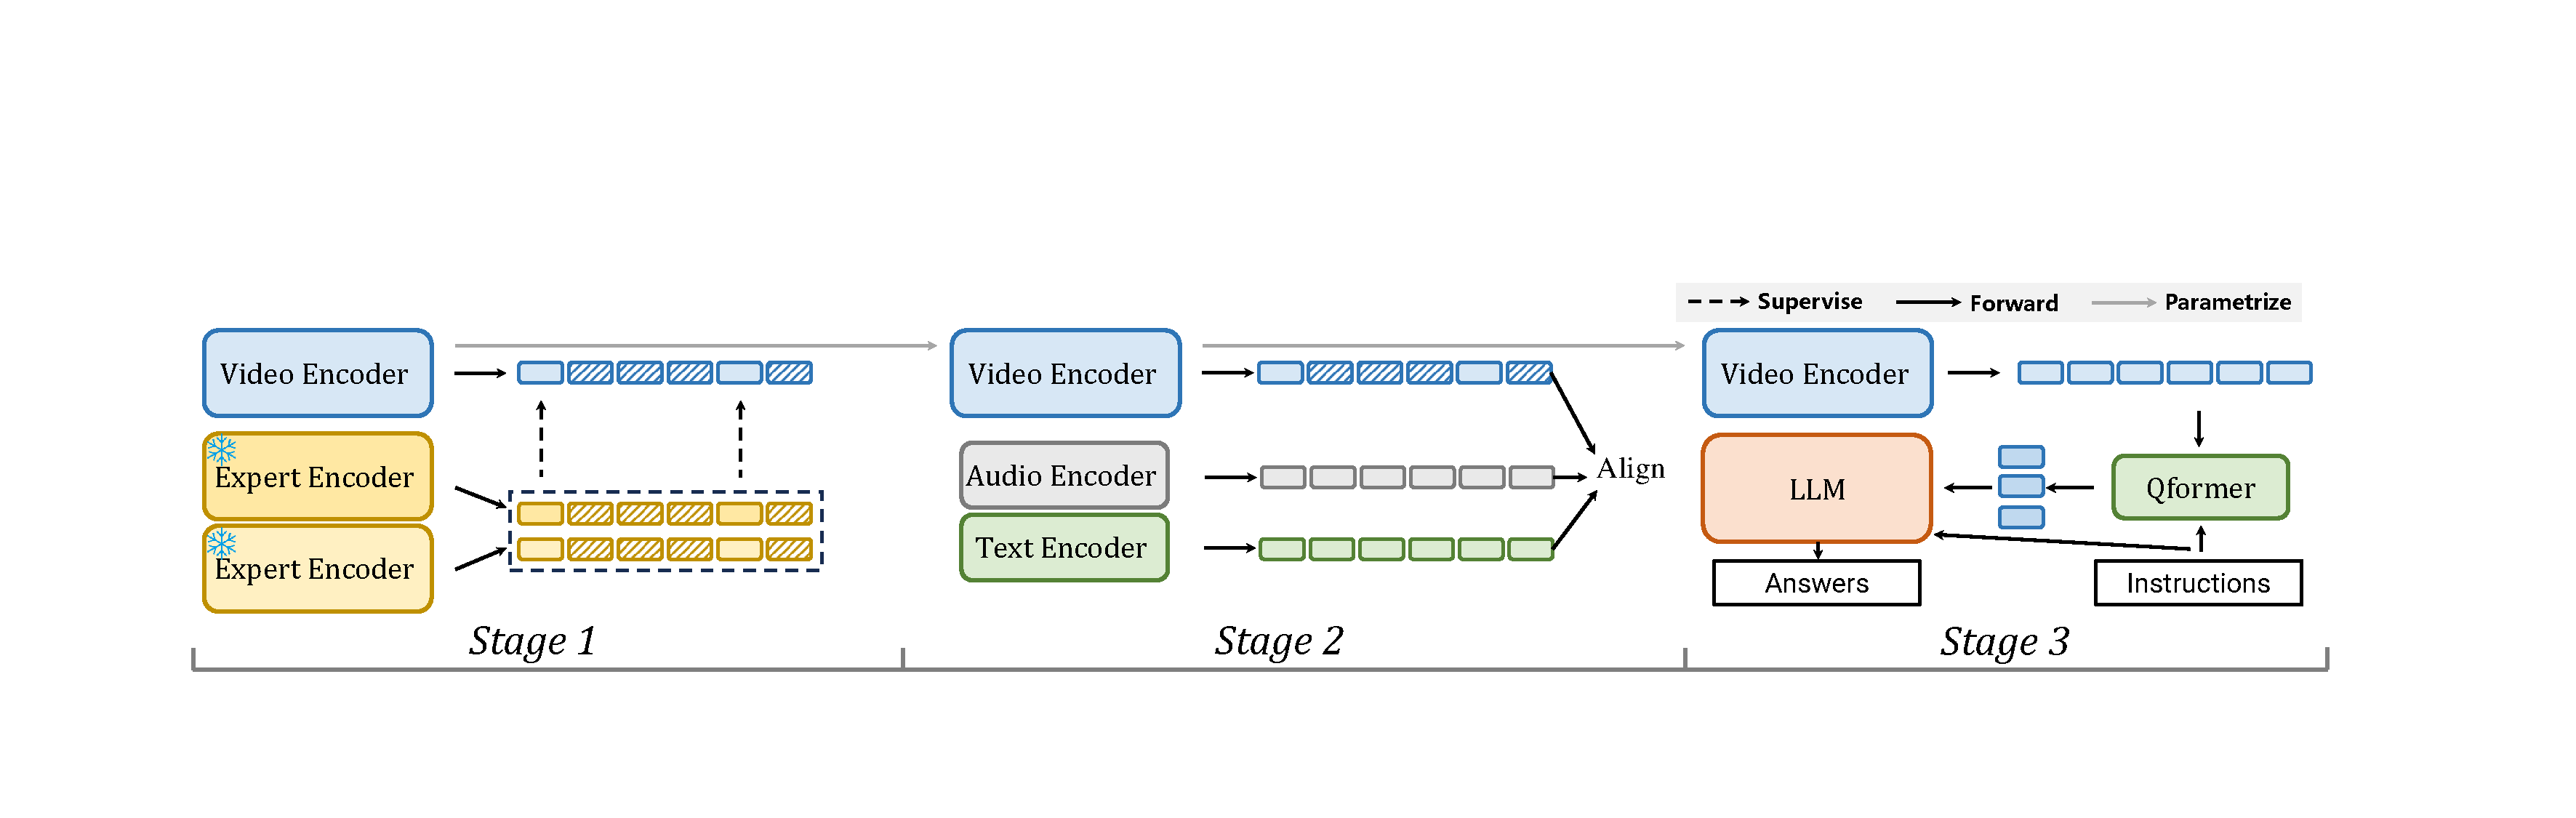
\includegraphics[width=1\textwidth]{content/figures/frame-v3.pdf}
    \vspace{-0.3cm}
    \caption{Framework of {\modelname}. It consists of three consecutive training phases: unmasked video token reconstruction, multimodal contrastive learning, and next token prediction. In stage 1, the video encoder is trained from scratch, while in stages 2 and 3, it is initialized from the version used in the previous stage.
    }
    \vspace{-3mm}
    \label{fig:frame}
\end{figure*}

\section{Method} \label{sec:method}

We learn {\modelname} in three stages, illustrated in Fig. \ref{fig:frame}. The stages include spatiotemporal token reconstruction, video-audio-speech-language contrastive learning, and connecting to a large language model (LLM) for joint training.

% \vspace{-2mm}
\paragraph{Video Encoder.} The video encoder used in {\modelname} follows the Vision Transformer (ViT) \cite{dosovitskiy2020image} and includes additional projection layers for distillation. Inspired by previous works \cite{chen2023internvl,coca}, we introduce attention pooling to the ViT.
For input videos, we sparsely sample 8 frames~\cite{tsn} and perform a 14$\times$14 ($h \times w$) spatial downsampling. These spatiotemporal tokens are then concatenated with a class token and combined with 3D position embeddings. The details of ViT-6B architecture are given in Supp.

\subsection{Stage1: Reconstructing Unmasked Video Tokens}

We exploit two expert models to guide the video encoder to conduct token-level reconstruction for unmasked areas.
Specifically, we adopt InternVL-6B~\cite{chen2023internvl} and VideoMAEv2-g~\cite{wang2023videomae} to transfer unmasked knowledge via simple projection layers. 
When training, we input the full videos into different teachers and mask out 80\% of the tokens frame by frame, under the semantic guidance of the multimodal model InternVL and motion-aware model VideoMAEv2. We only align the unmasked tokens, by minimizing their mean squared error (MSE) between student and teachers. The learning objective is to reconstruct the remaining tokens as:
\begin{equation}
    \mathcal{L} = \frac{1}{Z}\sum_{}{(\alpha_1|f^V(\mathbf{V}_p)-h(\mathbf{V}_p)|^2+\alpha_2|f^V(\mathbf{V}_p)-g(\mathbf{V}_p)|^2)},
\end{equation}
where $f^V$, $h$, and $g$ are our video encoder, InternViT-6B~\cite{chen2023internvl}, and ViT-g of VideoMAEv2, respectively. $p$ stands for the token index and $f(\mathbf{V}_p)$ is the corresponding token extracted by {\modelname} for input video $\mathbf{V}$. $Z$ is the normalization factor. $\alpha_1$ and $\alpha_2$ balance the influence between the employed models.

In our implementation, we randomly initialize the video encoder and then align its outputs from different layers (transformed by learnable multilayer perceptrons) to those of expert models. Specifically, we align: 1) the last $6$ layers of InternVL, 2) the last $4$ layers of VideoMAEv2, and 3) the final output token of InternVL. These alignments are made to the corresponding outputs of the video encoder using the $l_2$ norm. The different loss terms are simply summed for optimization. After pretraining, we drop those projection layers and only use the basic encoder. Compared with only using the multimodal model in UMT and VideoPrism, our strategy makes the vision encoder multimodal-friendly as well as enhances its temporal sensitivity for action modeling.


\subsection{Stage 2: Aligning Video to Audio-Speech-Text}

We exploit the correspondence between video and audio, speech, and text to encourage {\modelname} to learn more semantics. 
In practice, {\modelname} has a huge video encoder, and its employed audio and text encoders are relatively lightweight. The used audio encoder is a 12-layer transformer initialized with BEATs~\cite{beats} (90M). It takes as input 64-dimensional log Mel filterbank spectrograms, generated using a 25ms Hamming window, from 10-second-long clips (padded with zeros).
For the text and speech encoders, we initialize the text encoder and multimodal decoder using BERT-Large~\cite{devlin2018bert}. Specifically, we utilize the initial 19 layers of BERT-Large as the text encoder, with the subsequent 5 layers equipped with cross-attention layers serving as the multimodal decoder.

For pretraining objectives, we establish alignment across different modalities via text, including video, audio, image, and speech. We employ crossmodal contrastive and matching losses with masked language reconstruction loss as:
\begin{equation}
    \mathcal{L} = \mathcal{L}_\text{CON} + \mathcal{L}_\text{MAC} + \mathcal{L}_\text{MLM},
\end{equation}
The employed $\mathcal{L}_\text{MAC}$ and $\mathcal{L}_\text{MLM}$ are standard loss from \cite{Cheng2022VindLUAR}. Specifically, the crossmodal contrastive learning is given as:

\noindent\resizebox{\linewidth}{!}{%
\begin{minipage}{\linewidth}
\begin{align}
\resizebox{1\linewidth}{!}{
$\mathcal{L}_{\text{CON}} = \sum_{M, T_{M'}}\mathcal{L}_{\text{CON}}(M, T_{M'}) = -\sum_{M, T_{M'}} \left( \sum^N_{i=1} \log \frac{\exp(\text{sim}(f^{M}_i, f^{T_{M'}}_i) / \tau)}{\sum^N_{j=1} \exp(\text{sim}(f^{M}_i, f^{T_{M'}}_j) / \tau)} + \sum^N_{i=1} \log \frac{\exp(\text{sim}(f^{T_{M'}}_i, f^{M}_i) / \tau)}{\sum^N_{j=1} \exp(\text{sim}(f^{T_{M'}}_i, f^{M}_j) / \tau)} \right)$,}
\end{align}
\end{minipage}
}
\label{eq:loss_contrastive}
where $f^{V}$ and $f^{T}$ denote the learned video and text embeddings, respectively. $M$ and $T_{M'}$ indicates the modality of input signals and the text descriptions describing, respectively.
%and $M \in \{V, A, S, VA, VS, AS, VAS\}$ 
$\text{sim}(\cdot)$ computes the cosine similarity between two features. $\tau$ is the learnable temperature.

% \iffalse
For the matching part, it is given as:
\begin{equation}
    \mathcal{L}_{\text{MAC}} = - y \log f_p(\mathbf{V}, \mathbf{T}) - (1-y)\log (1-f_p(\mathbf{V}, \mathbf{T})),
\end{equation}
where $f_p(\mathbf{V}, \mathbf{T})$ computes the matching likelihood between $\mathbf{V}$ and $\mathbf{T}$. $y$ denotes whether the given video and text are paired ($y=1$) or not ($y=0$).

The employed masked language modeling loss is:
\begin{equation}
    \mathcal{L}_{\text{MLM}} = - \log f_p^T(\mathbf{T}_j|\mathbf{T}_{<j}),
\end{equation}
where $f_p^T(\mathbf{T}_j|\mathbf{T}_{<j})$ computes the likelihood of the $j_\text{th}$ text token based on the previous ones. Here $\mathbf{T}$ refers to video captions.
% \fi

To improve the training efficiency, we employ the masked learning strategy, aligning unmasked video tokens to tokens from other modalities first, then using full video tokens reconstruction shortly. Specifically, it consists of two steps as follows:

% \vspace{-2mm}
\paragraph{Aligning Masked Visual-Language-Audio.}
We freeze the audio encoder and focus on aligning visual, audio, and text features. For pre-training, we use a comprehensive set of image, video, and audio-video data. The combinations of modalities used are represented as $\{M, T_{M'}\} \in \{ \{I, T_I\}, \{V, T_V\}, \{V, T_\textit{VAS}\}, \{\textit{VA}, T_\textit{VAS}\}\}$ where each pair denotes the concatenated features from the respective modalities.

% \vspace{-2mm}
\paragraph{Unmasked Visual-Audio-Language Post-Pretraining.}
We freeze the vision encoder to jointly align audio, visual, and text features. Post-pretraining is conducted using a smaller subset of image and video data (25M samples), along with the full set of audio (0.5M samples) and audio-video data (50M samples). Since the parameters of the largest ViT-6B model are frozen, we do not use masking strategies in this phase to ensure consistency with the inference process and to minimize any performance degradation in downstream tasks. The modality combinations used here are $\{M, T_{M'}\} \in \{ \{I, T_I\}, \{V, T_V\}, \{A, T_{A}\}, \{V, T_\textit{VAS}\}, \{\textit{VA}, T_\textit{VA}\}\}\}$.

% \vspace{-2mm}
\subsection{Stage3: Predicting Next Token with Video-Centric Inputs}
% \vspace{-2mm}
To further enrich the semantics embedded in {\modelname} and improve its support for video-centric dialogue, we tune it by connecting it to a LLM with QFormer design~\cite{blip2,blip}. We employ the progressive learning scheme in \cite{li2023mvbench} by using \modelname{} as the video encoder and train a video blip for communicating with open-sourced LLM~\cite{vicuna,mistral}. 
Additionally, we implement a high-definition post-training stage to improve the model's fine-grained and long spatiotemporal capabilities. During this stage, the input video is divided into up to six sub-videos with a resolution of 224x224 pixels each, along with one global resized sub-video of the same resolution. We then train the model for two additional epochs: the first epoch uses 8-frame video inputs, while the second epoch uses 16-frame inputs.
During the additional training process, we update the video encoder and BLIP Qformer, while the LLM is updated using LoRA \cite{lora}.

% Please add the following required packages to your document preamble:
% \usepackage{multirow}
\begin{table}[t]
\centering
% \vspace{-3mm}
\caption{Summary of datasets used in \modelname{} pretraining process.}
% \vspace{-3mm}
\resizebox{0.8\textwidth}{!}
{
\begin{tabular}{cllcl}
\toprule
Pretraining Stage & {Dataset}                         & Domain            & \# of clips & Annotation            \\ \midrule
\multicolumn{1}{c|}{Stage 1} & KMash & Web Video & 2M & - \\
\midrule
\multicolumn{1}{c|}{Stage 2 (img-txt)} & LAION, etc & Web Image & 300M & Alt-text / Generated Caps \\
\hline
\multicolumn{1}{c|}{\multirow{4}{*}{Stage 2 (vid-txt)}} & WebVid2M     & Web Video         & 250k        & Alt-text               \\
\multicolumn{1}{c|}{}                              & WebVid10M    & Web Video         & 9.7M        & Alt-text               \\
\multicolumn{1}{c|}{}                              & InternVid    & Youtube Video     & 40M         & Generated Caption     \\
\multicolumn{1}{c|}{}                              & InternVid2 & Youtube Video     & 50M         & Generated Caption     \\ 
\midrule
\multicolumn{1}{c|}{Stage 3} & LLaVA, etc  & Web Image/Video         & 2.1M        & Conversation, QA  \\
\bottomrule
\end{tabular}
}
\label{tab:pretrain_data}
% \vspace{-3mm}
\end{table}
\vspace{-2mm}
\section{Multimodal Video Data}
\vspace{-3mm}
We list our training data in Tab. \ref{tab:pretrain_data}. Among the datasets used, KMash and InternVid2 are newly built, whereas the rest are publicly available.

\subsection{Video-only Data for Masked Autoencoders}
We curate a new video set without labels named \textit{K-Mash} from action recognition datasets~\cite{k400,sth,mit,activitynet,hacs}, as detailed in Supp. It encompasses a wide range of video types, including first- and third-person perspectives, with both short and long duration, and featuring various settings. Further, we give K-Mash$_{2M}$ with additionally sourced and selected 844K videos from YouTube for diversity. 

\begin{figure*}[t]
    \centering
    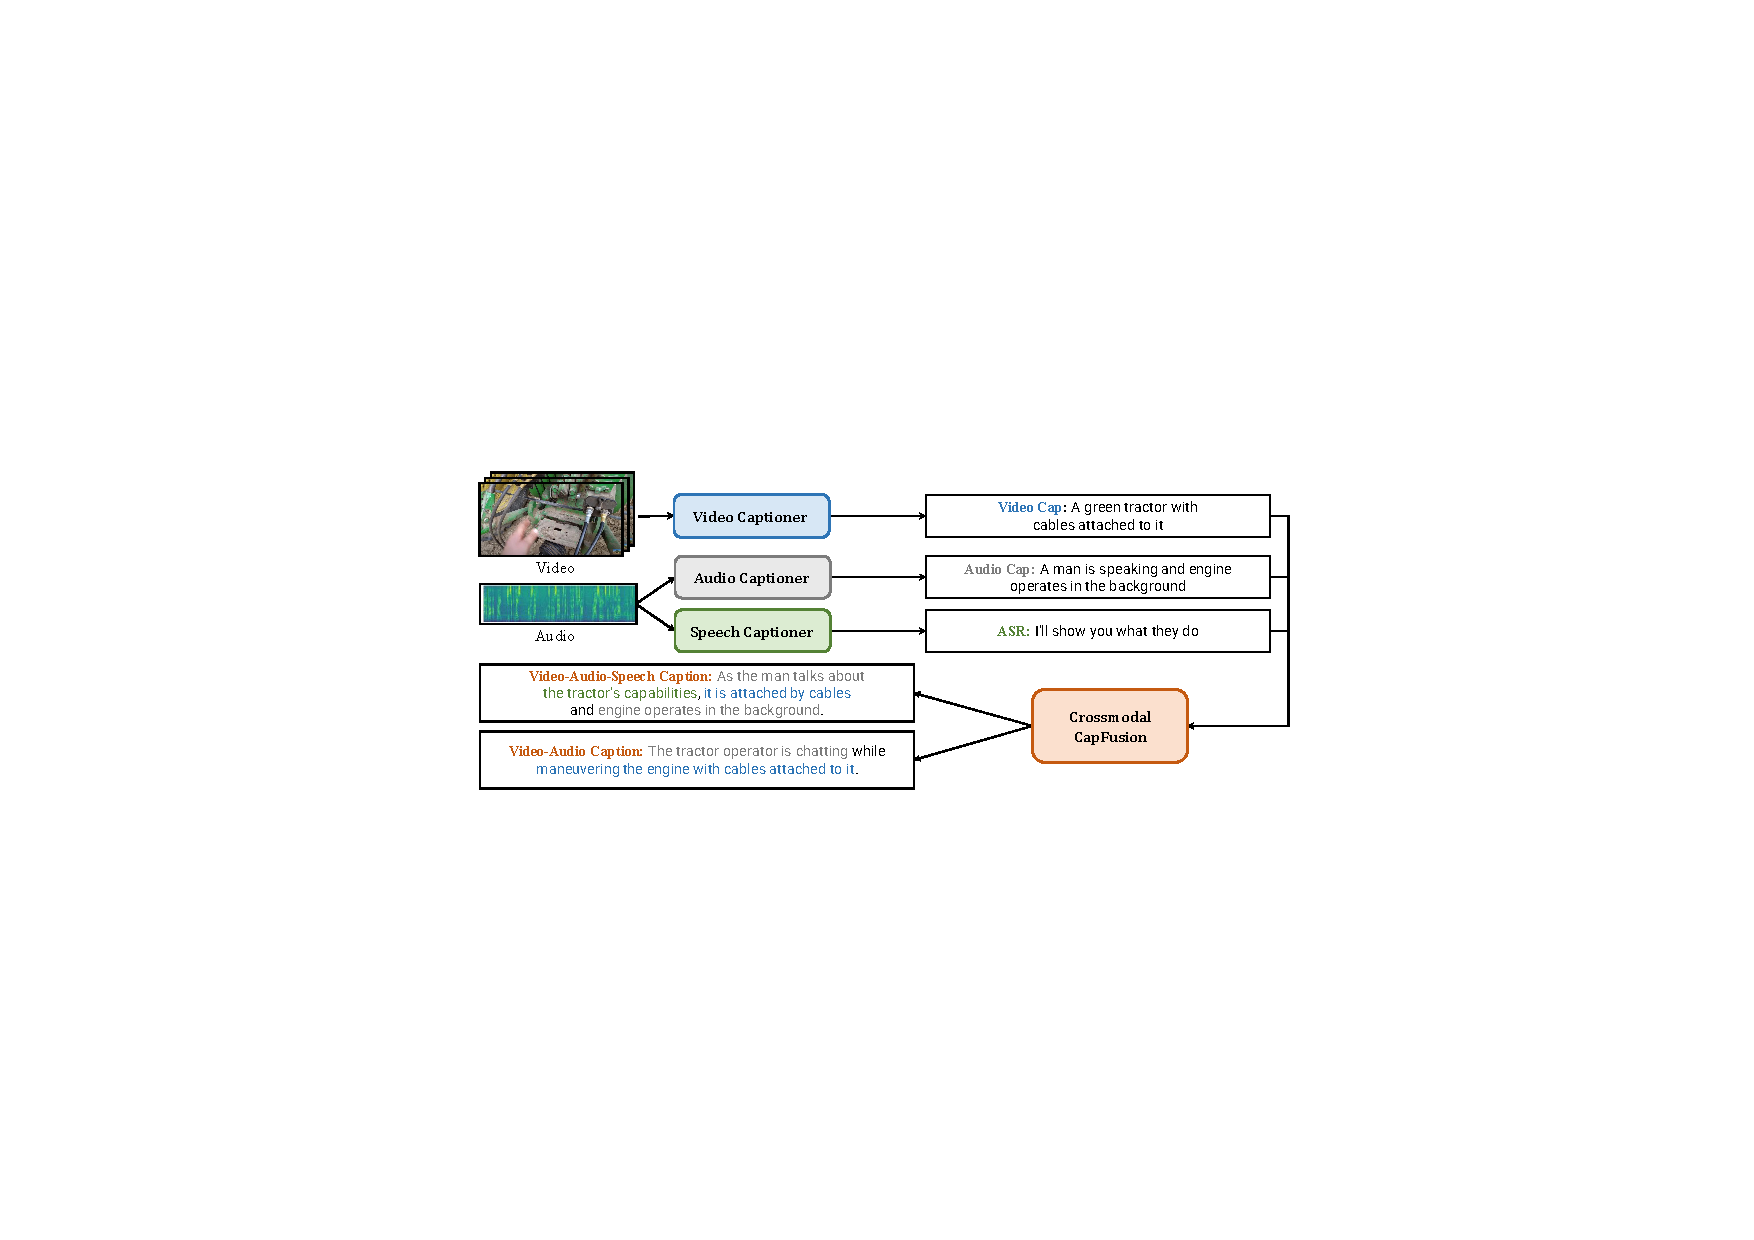
\includegraphics[width=0.9\textwidth]{content/figures/avs-autocap-v3.pdf}
    % \vspace{-0.3cm}
    \caption{The framework of our video multimodal annotation system, called {\annoname}, consists of four main components: video, audio, and speech captioners, along with a LLM for integrating captions from these modalities.}
    % \vspace{-3mm}
    \label{fig:anno}
\end{figure*}

% \vspace{-3mm}
\subsection{Videos with Audio-Speech Modalities}

We build a multimodal video dataset, coined as~{\dataname}, with video-audio-speech information and their descriptions for strengthening video perception via other modalities. It consists of 100M videos along with their VAS captions. 
In {\dataname}, we collect videos from several sources (detailed in the supp), segment them into clips, and automatically annotate them based on their unimodal or crossmodal inputs. We highlight the importance of temporal segmentation in clip generation and our video mutimodal annotation system. We find refining them leads to notable downstream improvements.  


\paragraph{Temporal Consistency Matters.} We employ a temporal boundary detection model AutoShot~\cite{zhu2023autoshot} to segment videos into clips instead of SceneDet filter from FFmpeg. It predicts  boundaries based on temporal semantic variations rather than pixel differences, and is able to generate semantically complete cuts without mixing extra frames with inconsistent context. 

\paragraph{Video Multimodal Annotation.} We design a video multimodal annotation system {\annoname} to give proper unimodal and crossmodal descriptions for textualizing videos from different perceptions. It automatically captions visual, audio, and speech of {\dataname}, then it corrects them and fuses them for cross-modal captions via LLM. The system frame is given in Fig. \ref{fig:anno}. {\annoname} has independent video, audio, speech captioner, and a LLM for caption refinement and fusion. For video, speech, and caption postprocessing, we employ existing methods as the video captioning pipeline in \cite{wang2023internvid}, WhisperV2-large model~\cite{whisper}, and Vicuna-1.5~\cite{vicuna}. For audio, we craft a audio captioner upon VideoChat~\cite{li2023videochat}, as we find no open-sourced one. It extracts audio features from inputs by Beats~\cite{beats}. We learn it by only tuning its Qformer using a combination of the large-scale audio-text corpus WavCaps~\cite{mei2023wavcaps} dataset. Details are given in the supplementary material. 

\subsection{Instruction-Tuning Data for Video Dialogue}
% \label{sec:instruction_data}
We employ a updated training version of MVBench \cite{li2023mvbench}. Originally, it comprises 1.9M samples (both images and videos) from 34 distinct sources. We decrease the amount of caption data from WebVid and CoCo to 80k and 100k separately and add new data from the S-MiT to boost the diversity rather than quantity of the instruction dataset. In the additional HD training stage, we incorporate the videos with corresponding GPT-4 annotations from \cite{chen2024sharegpt4video} into the training set. We further expand the training set by including datasets from PerceptionTestQA \cite{perceptiontest}, TVQA \cite{tvqa}, NTU-RGB-D \cite{ntu_rgbd}, and EgotaskQA \cite{ego4d}, along with grounding datasets based on DiDeMo \cite{didemo} and COCO \cite{coco}.
This training data encompasses key features of image and video understanding across crucial tasks, including 1) conversation, 2) caption, 3) visual question answer, 4) reasoning, and 5) classification. 
